% Modified for use with IJQC - Madhusudan Singh Copyright (C) (2011). All rights reserved.
\documentclass[12pt]{article}

\setlength{\oddsidemargin}{0in}  %left margin position, reference is one inch
\setlength{\textwidth}{6.5in}    %width of text=8.5-1in-1in for margin
\setlength{\topmargin}{-0.5in}    %reference is at 1.5in, -.5in gives a start of about 1in from top
\setlength{\textheight}{9in}     %length of text=11in-1in-1in (top and bot. marg.) 
\newenvironment{wileykeywords}{\textsf{Keywords:}\hspace{\stretch{1}}}{\hspace{\stretch{1}}\rule{1ex}{1ex}}

\usepackage{amsmath,amssymb}
\usepackage{graphicx}% Include figure files
\usepackage{caption}
\usepackage{bm}
\usepackage{color}% Include colors for document elements
\usepackage{dcolumn}% Align table columns on decimal point
\usepackage[numbers,super,comma,sort&compress]{natbib}

\usepackage{soul}

\definecolor{background-color}{gray}{0.98}
\graphicspath{{data/}{images/}}

%\title{Atomic pseudo-potentials for sp$^2$ carbon atoms}
\title{Graphical abstract}

\begin{document}
\maketitle
\begin{figure}[h]
\centering
\colorbox{background-color}{
\fbox{
\begin{minipage}{1.0\textwidth}
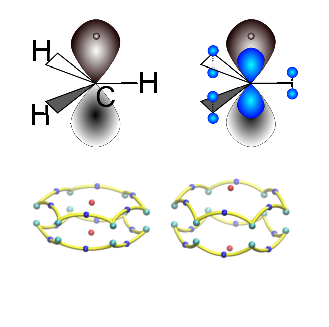
\includegraphics[width=50mm,height=50mm]{graphical_abstract.eps} % Pick only one of the two styles by uncommenting the corresponding \includegraphics
%\includegraphics[width=110mm,height=20mm]{cc.eps}
A pseudo-potential system for an sp\(^{2}\) carbon atom is built and tested as a building block for various pseudo-hydrocarbon polyenes and polycyclic aromatic hydrocarbons.  
It is employed in \textsl{ab-initio} calculations in which several physical characteristics are found to be well-reproduced by the pseudo-system. 
This approach is capable of reproducing the $\pi$ electron systems of planar hydrocarbons at low computational cost.
\\
\end{minipage}
}}
\end{figure}

\end{document}
